% This is samplepaper.tex, a sample chapter demonstrating the
% LLNCS macro package for Springer Computer Science proceedings;
% Version 2.20 of 2017/10/04
%
\documentclass[runningheads]{llncs}
%
\usepackage{graphicx}

\begin{document}
%
\title{Cloud Based Automation}

\author{Group Name: Sandesh Kenjana Ashok \and
Mirac Coskuner \and
Kartik Nayak}

\institute{Service Computing Department, IAAS, University of Stuttgart
\email{st164259@stud.uni-stuttgart.de}, \email{st100147@stud.uni-stuttgart.de},  \email{st164247@stud.uni-stuttgart.de}}
%
\maketitle              % typeset the header of the contribution
%
\begin{abstract}
Automated infrastructural technology is coming age of technology. Using smart infrastructural technology with an intent to conserve power can lead to energy efficiency, savings, and an overall better quality of life. Suppose, having air conditioning turn on when the user walks into the house. It is comfortable, but the air conditioning turn off when the user leaves the house is energy saving. This application uses the power of internet of things to make decisions pertaining to energy efficiency, providing the benefits in terms of comfort, safety, health and encouraging productivity at both home and workplace. The project intends to provide a connected experience between home and workplace through a messaging queue.


\keywords{Smart Home  \and Smart Workplace \and Energy management \and Comfort.}
\end{abstract}
%
%
%
\section{Introduction}
The application is developed with an intention to reduce the power consumption at both home and workplace without compromising on the user experience. The participatory sensors sense the presence of users in the provided environment to enable the benefits suitable for the situation. However the user can override the decision made by the system through Google Assistant's voice commands. Since both home and workplace are controlled in the application, the raspberry pi controllers are placed at both locations and have a shared a messaging queue that provides a seamless experience for the user. At home environment, with the available sensors and actuators, lamp and heater are controlled based on  environmental light and environmental temperature. At workplace environment, computer monitor power socket and in-place light are controlled based on user's presence. The sensor values are displayed on the dashboard in real time. With an intent of sustainability, the application aims to conserve the energy, also providing the user comfort and better quality of life. 



\section{System Design}
\begin{figure}
        \centering
        \includegraphics[width=1\textwidth]{Home_System_Architecture.png}
        \caption{Home System Architecture}
        \label{fig:correctness}
    \end{figure}
Fig. 1 and Fig. 2 show the home system architecture and workplace system architecture respectively. In the home system architecture, the raspberry pi is connected physically to the GrovePi+ board, Plugwise USB stick, mic and speakers. The libraries of Paho MQTT client, Plugwise and GrovePi are installed in the python environment, and Google Assistant API is configured. As shown in Fig. 3, based on the light sensor and temperature sensor, lamp and heater are controlled. But user can override these actuation with his/her voice input. To eliminate the confusion between sensor actuation and Google Assistant input, a socket is introduced (as shown in Fig. 1) between the functions for communication, with Google Assistant having higher priority. Both these functions in the application layer from Fig. 1 instruct the raspberry pi controller unit to send actuation signals to plugwise circle+ and circle plugs that are communicating with the plugwise stick over zigbee protocol. The sensor data and the status of the actuators are pushed to the MQTT cloud and are displayed in the Thingsboard dashboard in real time. The paho client acts as a publisher in the home environment.
\begin{figure}
        \centering
        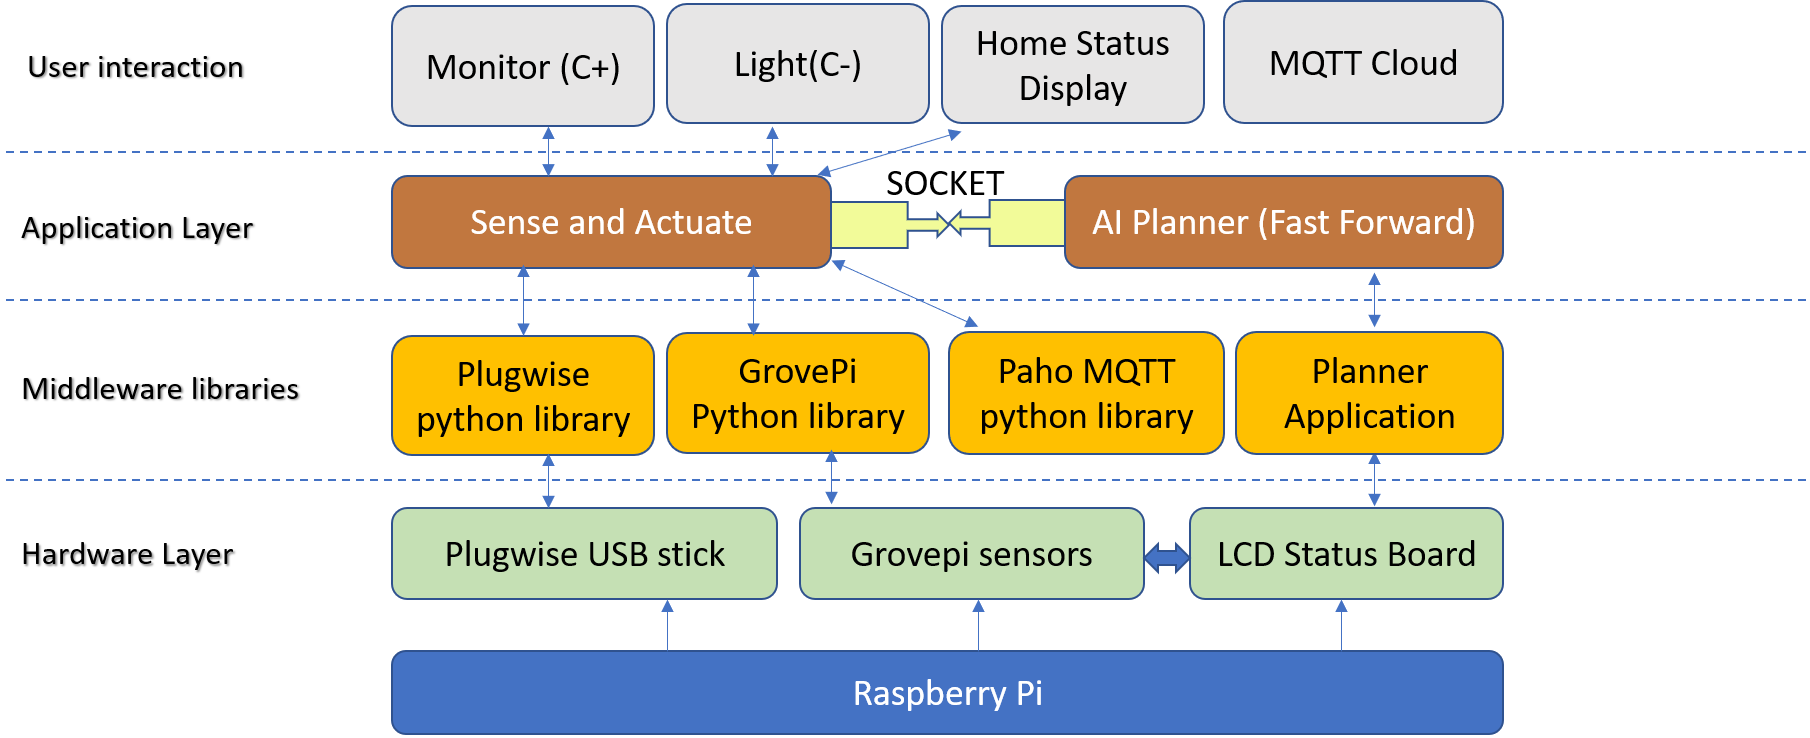
\includegraphics[width=1\textwidth]{Office_System_Architecture.png}
        \caption{Workplace System Architecture}
        \label{fig:correctness}
    \end{figure}
\newline
In the workplace system architecture, the paho MQTT client acts as a subscriber. It gathers the status of lamp and heater from home environment and displays it on the LCD board placed at the desk in the workplace environment. The sensor inputs are read from sound and ultrasound sensors and are fed to both the functions in the application layer of Fig. 2. The AI planner generates the suitable actions to be taken and communicates it to the Sense and Actuate function which instructs the raspberry pi to wirelessly control plugwise modules.



\section{Set up and implementation}
\begin{figure}
  \centering
  \begin{minipage}[b]{0.55\textwidth}
    \includegraphics[width=\textwidth]{homedesign.png}
    \caption{Home setup}
  \end{minipage}
  \hfill
  \begin{minipage}[b]{0.4\textwidth}
    \includegraphics[width=\textwidth]{workplacedesign.png}
    \caption{Workplace setup}
  \end{minipage}
\end{figure}

\begin{figure}
        \centering
        \includegraphics[width=1\textwidth]{overalldesign.png}
        \caption{overall setup}
        \label{fig:correctness}
    \end{figure}
For energy efficiency and comfort, the sensors are placed at both home and workplace, and in addition the home environment is facilitated with Google Assistant. For the execution of the design, both environments have a raspberry pi controller each which are connected to each other over MQTT messaging queue. In the home environment, the raspberry pi hosts a GrovePi+ board, senses for light and temperature, gathered from light sensor and temperature sensor connected to port 0 and port 4 of the GrovePi+ board respectively, and the inputs are processed in a rule based planning to take necessary actions. Light and temperature sensors used are GrovePi sensors and they are configured as described in ~\cite{1}. Furthermore, the experience in the environment is enriched with the Google Assistant API which is enabled by registering the devices in the Google Developers platform ~\cite{ref_url1}. The custom phrases for controlling both lamp and heater through Google Assistant are integrated in the python script to eliminate ambiguity. Based on the light available in the environment, the lamp would be controlled to provide optimal brightness in the environment. Likewise, the heater is controlled based on the inputs from temperature sensor to provide a conducive living experience. However, the user has freedom to control both lamp and heater, and he/she can do so with the help of Google Assistant that will overwrite the actuation from sensors inputs. The block diagram of the home set up is shown in Fig. 3. \newline
\newline
In the workplace environment, as shown in Fig. 4,  the raspberry pi controller senses for the user presence through sound sensor and ultrasound sensor (GrovePi sensors) connected to port 0 and port 2 of the GrovePi+ board, that's mounted on raspberry pi controller,  respectively. The sensor values are processed by fast forward AI planner as described in ~\cite{ref_article1}. The AI planner generates the planning, and it is communicated to the sensing and actuating function that parses the planning. The actuators controlled in the environment are computer monitor and in-place light, both of which are controlled based on the combined inputs from sound and ultrasound sensors.\newline
\newline
Both the raspberry pi controllers are configured with paho MQTT client, and the client in the home environment acts as publisher while the one in the workplace environment acts as subscriber as shown in Fig. 5. CloudMQTT broker has been configured. Paho client from home environment sends the sensor data and the status of lamp and heater to CloudMQTT, and the paho client of workplace environment subscribes to the status of lamp and heater and displays it on the LCD panel implemented at the user's desk at the workplace. The sensor values and the status of actuators are displayed on Thingsboard dashboard in real time~\cite{ref_url2}. All the actuators are controlled by plugwise smart plugs that communicate over zigbee protocol~\cite{2}. 


\section{Conclusions and Outlook}
With this application,we plan to minimize the unproductive expenditure of the power, also prioritizing on user comfort. With the available sensors, actuators and controllers, the application could control lamp and heater at home and computer monitor power socket and in-place light at workplace. The dashboard, that employs the message queue, shows sensor data to the user in real time. The concept could be extended where a user gets an alert on his smartphone or smart watch when there is an unnecessary leak of power, say refrigerator door is unlocked in the kitchen, the user can get an SMS on his/her cellphone in the bedroom. This strategy will notify the user whenever there is unnecessary wastage of power that wouldn't have a simple solution by turning the power socket off. Such smart systems can provide guidelines for preserving power. Thus the proposed application can be extended for the betterment of the society.

%
% ---- Bibliography ----
%
\bibliographystyle{splncs04}
\bibliography{mybib}



\end{document}

